\documentclass[tikz,border=2pt]{standalone}
\usepackage{amsmath,amssymb}
\usetikzlibrary{arrows.meta,decorations.pathreplacing}
\begin{document}
% Nine jobs with three non-preemptive outages in both rows: planned setups every B=3 jobs (top)
% versus random adjustments after each job with probability p=1/3 (bottom), where the numbers of
% jobs between adjustments are 3, 5 and 1 (first-success counts with mean 1/p=3).
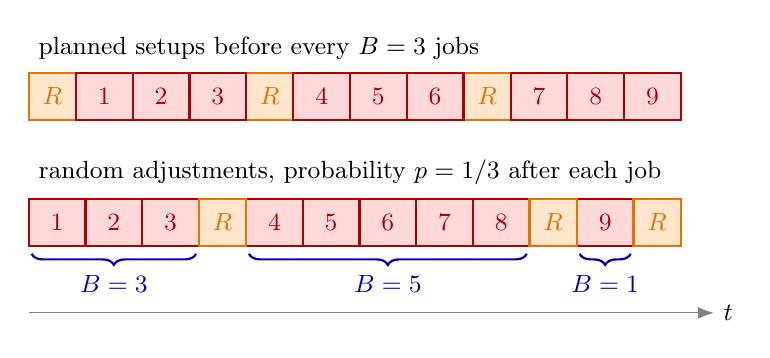
\begin{tikzpicture}[font=\small, >={Latex[length=2mm]}, x=1.2cm, y=1cm]
  \tikzset{job/.style={draw=red!70!black, fill=red!15, thick},
           outage/.style={draw=orange!90!black, fill=orange!20, thick}}
  % top row: planned setups
  \node[anchor=south west] at (0,2.25) {planned setups before every $B=3$ jobs};
  \foreach \a/\b in {0/0.5, 2.3/2.8, 4.6/5.1} {
    \draw[outage] (\a,1.6) rectangle (\b,2.2);
    \node[orange!90!black] at ({(\a+\b)/2},1.9) {$R$};
  }
  \foreach \a/\k in {0.5/1, 1.1/2, 1.7/3, 2.8/4, 3.4/5, 4.0/6, 5.1/7, 5.7/8, 6.3/9} {
    \draw[job] (\a,1.6) rectangle (\a+0.6,2.2);
    \node[red!70!black] at (\a+0.3,1.9) {$\k$};
  }
  % bottom row: random adjustments
  \node[anchor=south west] at (0,0.65) {random adjustments, probability $p=1/3$ after each job};
  \foreach \a/\k in {0/1, 0.6/2, 1.2/3, 2.3/4, 2.9/5, 3.5/6, 4.1/7, 4.7/8, 5.8/9} {
    \draw[job] (\a,0) rectangle (\a+0.6,0.6);
    \node[red!70!black] at (\a+0.3,0.3) {$\k$};
  }
  \foreach \a/\b in {1.8/2.3, 5.3/5.8, 6.4/6.9} {
    \draw[outage] (\a,0) rectangle (\b,0.6);
    \node[orange!90!black] at ({(\a+\b)/2},0.3) {$R$};
  }
  % numbers of jobs between adjustments
  \draw[decorate, decoration={brace, amplitude=4pt, mirror}, blue!70!black, thick] (0.03,-0.1) -- (1.77,-0.1)
    node[midway, below=4pt] {$B=3$};
  \draw[decorate, decoration={brace, amplitude=4pt, mirror}, blue!70!black, thick] (2.33,-0.1) -- (5.27,-0.1)
    node[midway, below=4pt] {$B=5$};
  \draw[decorate, decoration={brace, amplitude=4pt, mirror}, blue!70!black, thick] (5.83,-0.1) -- (6.37,-0.1)
    node[midway, below=4pt] {$B=1$};
  % time axis
  \draw[->, gray] (0,-0.85) -- (7.25,-0.85) node[right, black] {$t$};
\end{tikzpicture}
\end{document}
